% Fakesection 序言之前

\RequirePackage[l2tabu, orthodox]{nag}
\RequirePackage{ifxetex}
\RequireXeTeX
\documentclass{ctexart}

%颜色
\usepackage{xcolor}

%长度
\usepackage{printlen}
\uselengthunit{mm}

%图形
\usepackage{media9}
\usepackage{pdfpages}
\usepackage{overpic}
\usepackage{graphicx}
\graphicspath{{./src/}}
\usepackage{wallpaper}
\usepackage{wrapfig}
\usepackage{pstricks}
\usepackage{smartdiagram}
\usepackage[edges]{forest}
\usepackage{pgfplots}
\usepackage{tikz}
\usetikzlibrary{shapes.geometric}
\usetikzlibrary{calc}
\usetikzlibrary{patterns}
\usetikzlibrary{arrows}
\usetikzlibrary{shapes}
\usetikzlibrary{chains}
\usetikzlibrary{mindmap}
\usetikzlibrary{graphs}
\usetikzlibrary{decorations.text}
\usetikzlibrary{arrows.meta}
\usetikzlibrary{shadows.blur}
\usetikzlibrary{shadings}
\usepackage{scsnowman}
\usepackage{tikzpeople}
\usepackage{tikzducks}
\usepackage{pifont}
\usepackage{marvosym}
\usepackage{fontawesome}
\usepackage{stmaryrd}
\usepackage{ean13isbn}
\usepackage{qrcode}
\usepackage{pgf-pie}
\usepackage{pgfmath}

%表格
\usepackage{tabu}
\usepackage{longtable}
\usepackage{booktabs}
\usepackage{diagbox}
\usepackage{multicol}
\usepackage{multirow}
\usepackage{makecell}
\usepackage{fancybox}
\usepackage{colortbl}
\usepackage{tcolorbox}
\tcbuselibrary{skins}
\tcbuselibrary{breakable}
\tcbuselibrary{theorems}
\tcbuselibrary{listings}
\tcbuselibrary{xparse}
\usepackage{fvextra}
\usepackage{csvsimple}
\usepackage{boxedminipage2e}

%公式
\usepackage{amsmath}
\usepackage{amsthm}
\usepackage{amsfonts}
\usepackage{amssymb}
\usepackage{amsbsy}
\usepackage{amsopn}
\usepackage{amstext}
\usepackage{mathrsfs}
\usepackage{bm}
\usepackage{textcomp}
\usepackage{latexsym}
\usepackage{exscale}
\usepackage{relsize}
%\usepackage{xymtex}
\usepackage{physics}
\usepackage{siunitx}
\usepackage{hologo}
\usepackage{cases}

%正文
\usepackage{fancyhdr}
\usepackage{geometry}
\usepackage{lastpage}
\usepackage{indentfirst}
\usepackage{setspace}
\renewcommand\arraystretch{1.5}

%非正文
\usepackage{makeidx}
\makeindex
\usepackage{epigraph}
\usepackage{varwidth}

%参考文献
\usepackage{morewrites}
\renewcommand{\thefootnote}{\fnsymbol{footnote}}
\usepackage[resetlabels]{multibib}
\newcites{sec}{参考网站}

%%链接
\usepackage
[	colorlinks = true,
linkcolor = gray,
citecolor = gray,
backref=page
]{hyperref}
\usepackage{caption}
\usepackage{subcaption}

%其它
\usepackage{atbegshi}
\usepackage{lipsum}

%文字
\usepackage{csquotes}
\usepackage{microtype}

\csname
endofdump
\endcsname

%\usepackage[notref,notcite]{showkeys}

%%代码
\usepackage{minted}
\tcbuselibrary{minted}% 用minted排版代码
%Java %与mcode冲突
% \usepackage{lstcustom}
%Matlab %与lstcustom冲突
%\usepackage[framed,numbered,autolinebreaks,useliterate]{mcode}
%\usepackage{boxie}
%\makeatletter
%\xdefinecolor{tcbcol@back}{rgb}{0,0,0}
%\makeatother

%枚举%与beamer冲突
\usepackage{enumitem}
\setlist[enumerate, 2]
{	fullwidth,
	label = \alph*.,
	font = \textup,
	itemindent=2em
}

\usepackage{titlesec}
%\titleformat{\chapter}{\centering\Huge\bfseries}{实验\chinese{chapter}~}{4mm}{}
\titleformat{\section}{\heiti\zihao{4}\bfseries}{\ifthenelse{\value{section}=0}{}{\thesection}~}{0pt}{\vspace{12pt}}[\vspace{12pt}]
\titleformat{\subsection}{\heiti\zihao{-4}\bfseries}{\arabic{section}.\arabic{subsection}~}{0pt}{\vspace{6pt}}[\vspace{6pt}]
\titleformat{\subsubsection}{\zihao{-4}}{ (\arabic{subsubsection}) ~}{0pt}{}
\titleformat{\paragraph}{\zihao{-4}}{第\chinese{paragraph},}{0pt}{}

\begin{document}

% Fakesection 扉页

\begin{titlepage}
	\centering
	\makebox[4\ccwd][s]{}

	\vspace{40mm}
	\textbf{\fontsize{25pt}{\baselineskip}\kaishu{南京理工大学经济管理学院}}

	\vspace{5mm}
	\textbf{\fontsize{33pt}{\baselineskip}\lishu{课程论文}}

	\vspace{20mm}
	\begin{table}[htpb]
		\centering
		\songti
		\zihao{3}
		\begin{tabu}to.8\linewidth{@{}X[4,r]@{}X[c]@{}X[18,l]@{}}
			\makebox[4\ccwd][s]{课程名称}&:&\underline{\makebox[18\ccwd][c]{战略与风险管理}}\\
			\makebox[4\ccwd][s]{论文题目}&:&\underline{\makebox[18\ccwd][c]{以铱星计划为例的项目风险管理案例分析}}\\
			\makebox[4\ccwd][s]{姓名}&:&\underline{\makebox[18\ccwd][c]{吴振宇}}\\
			\makebox[4\ccwd][s]{学号}&:&\underline{\makebox[18\ccwd][c]{916101630117}}\\
			\makebox[4\ccwd][s]{成绩}&:&\underline{\makebox[18\ccwd][c]{}}\\
			\makebox[4\ccwd][s]{时间}&:&\underline{\makebox[18\ccwd][c]{\today}}
		\end{tabu}
	\end{table}
\end{titlepage}

% Fakesection 评分

\thispagestyle{empty}

\begin{boxedminipage}{\linewidth}
	\zihao{4}

	任课老师评语:

	\vspace{40mm}

	\begin{flushright}
		签名: \underline{\makebox[6\ccwd][c]{}}

		年\makebox[2\ccwd][c]{}月\makebox[2\ccwd][c]{}日
	\end{flushright}

	\vspace{20mm}

\end{boxedminipage}

% Fakesection 摘要

\title{\heiti\zihao{2}\textbf{以铱星计划为例的项目风险管理案例分析}}
\author{\kaishu\zihao{4}\textbf{916101630117~吴振宇} }
\date{}
\maketitle

{
	\setlength{\baselineskip}{18pt}
	\kaishu

	\renewcommand{\abstractname}{}
	\begin{abstract}
		\zihao{5}
		\noindent
		\textbf{摘要: }复杂多变的经营环境及市场经济中的各种不确定因素使得公司战略风险成为企业面临的最大的风险。不考虑竞争对手的反应及其一系列的攻击行为的传统静态竞争已经退出历史舞台,依靠各种战略取胜的动态竞争拉开帷幕。企业想要在复杂多变的环境中谋求生存发展甚至实现快速扩张,战略风险管理发挥着举足轻重的作用,战略决策的正确和风险管理的高效与否关系到企业的兴衰存亡。本文以铱星计划的失败案例作为分析对象,分析摩托罗拉公司在战略风险管理上的不足之处,并给出相关的建议。
	\end{abstract}

	\textbf{关键词:}战略投资;风险管理;铱星计划;摩托罗拉。

	\renewcommand{\abstractname}{}
	\begin{abstract}
		\zihao{5}
		\noindent
		\textbf{Abstract: }The complex and changeable business environment and various uncertain factors in the market economy make the strategic risk of the company the biggest risk faced by the enterprise. The traditional static competition, which does not take into account the reactions of competitors and a series of aggressive actions, has withdrawn from the historical stage, and the dynamic competition, which depends on various strategies to win, has begun. Enterprises want to seek survival, development and even rapid expansion in a complex and changeable environment. Strategic risk management plays an important role. The correct strategic decision-making and the efficient risk management are related to the rise and fall of enterprises. This paper takes the failure case of Iridium Planning as the object of analysis, analyses the shortcomings of Motorola in strategic risk management, and gives relevant suggestions.
	\end{abstract}

	\textbf{Key Words: }Strategic investment; Risk management; Iridium Planning; Motorola.
}

%页眉页脚%与book冲突
\pagestyle{fancy}
\renewcommand{\headrulewidth}{0pt}
\rhead{}
\lfoot{\small{\leftmark}}
\cfoot{\small{第\thepage 页~共~\pageref{LastPage}~页}}
\rfoot{\small{\rightmark}}

\setcounter{page}{1}

\section{引言}%
\label{sec:引言}

竞争形势的日益激烈使得公司日益重视发展战略的制定。战略投资存在的风险与收益的正比性也往往使许多企业担心一步失误全盘皆输,因此战略风险管理有其存在和研究的价值。\cite{2016企业战略与风险管理}

风险与收益往往是成正比的。分析一个战略的正确与否,不仅要看能取得的收益大小,更要分析其收益的可行性也就是风险的高低。为了获取看似客观的收益而铤而走险,往往会给企业带来意向不到的后果。

\begin{figure}[htpb]
	\centering
	\definecolor{ocre}{HTML}{800000}
	\definecolor{sky}{HTML}{C6D9F1}
	\definecolor{skybox}{HTML}{5F86B3}
	% arctext from Andrew code with modifications:
	%Variables: 1: ID, 2:Style 3:box height 4: Radious 5:start-angl 6:end-angl 7:text {format along path}
	\def\arctext[#1][#2][#3](#4)(#5)(#6)#7{
		\draw[#2] (#5:#4cm+#3) coordinate (above #1) arc (#5:#6:#4cm+#3)
		-- (#6:#4) coordinate (right #1) -- (#6:#4cm-#3) coordinate (below right #1) arc (#6:#5:#4cm-#3) coordinate (below #1)
		-- (#5:#4) coordinate (left #1) -- cycle;
		\def\a#1{#4cm+#3}
		\def\b#1{#4cm-#3}
		\path[
		decoration={
			raise = -0.5ex, % Controls relavite text height position.
			text  along path,
			text = {#7},
			text align = center,
		},
		decorate
		]
		(#5:#4) arc (#5:#6:#4);
	}
	%arcarrow, this is mine, for beerware purpose...
	%Function: Draw an arrow from arctex coordinate specific nodes to another
	%Arrow start at the start of arctext box and could be shifted to change the position
	%to avoid go over another box.
	%Var: 1:Start coordinate 2:End coordinate 3:angle to shift from acrtext box
	\def\arcarrow(#1)(#2)[#3]{
		\draw[thick,->,>=latex]
		let \p1 = (#1), \p2 = (#2), % To access cartesian coordinates x, and y.
		\n1 = {veclen(\x1,\y1)}, % Distance from the origin
		\n2 = {veclen(\x2,\y2)}, % Distance from the origin
		\n3 = {atan2(\y1,\x1)} % Angle where acrtext starts.
		in (\n3-#3: \n1) -- (\n3-#3: \n2); % Draw the arrow.
	}
	\begin{tikzpicture}[
		% Environment Cfg
		font=\sf    \scriptsize,
		% Styles
		myarrow/.style={
			thick,
			-latex,
		},
		Center/.style ={
			circle,
			fill=ocre,
			text=white,
			align=center,
			font =\footnotesize\bf,
			inner sep=1pt,
		},
		RedArc/.style ={
			color=black,
			thick,
			fill=ocre,
			blur shadow, %Tikzedt not suport online view
		},
		SkyArc/.style ={
			color=skybox,
			thick,
			fill=sky,
			blur shadow, %Tikzedt not suport online view
		},
		]
		% Drawing the center
		\node[Center](企业战略分析相关因素) at (0,0) {企业战略分析\\相关因素};
		\coordinate (企业战略分析相关因素-R) at (0:1.2); % To make compatible with \arcarrow macro.
		% Drawing the Tex Arcs
		% \Arctext[ID][box-style][box-height](radious)(start-angl)(end-angl){|text-styles| Text}
		\arctext[内部资源分析][RedArc][8pt](2.25)(180)(60){|\footnotesize\bf\color{white}|内部资源分析};
	\arctext[市场竞争能力][RedArc][8pt](2.25)(50)(-20){|\footnotesize\bf\color{white}|市场竞争能力};
\arctext[企业能力分析][RedArc][8pt](2.25)(190)(255){|\footnotesize\bf\color{white}|企业能力分析};
\arctext[经营环境分析][SkyArc][5pt](3.5)(205)(265){|\scriptsize\bf|经营环境分析};
\arctext[宏观环境分析][SkyArc][5pt](3.5)(270)(320){|\scriptsize\bf|宏观环境分析};
\arctext[行业环境分析][SkyArc][5pt](3.5)(-35)(20){|\scriptsize\bf|行业环境分析};
%Drawing the Arrows
%\arcarrow(above/below ID)(abobe/below ID)[shift]
\arcarrow(below 内部资源分析)(企业战略分析相关因素-R)[60];
\arcarrow(below 市场竞争能力)(企业战略分析相关因素-R)[30];
\arcarrow(below 企业能力分析)(企业战略分析相关因素-R)[-30];
\arcarrow(below 行业环境分析)(企业战略分析相关因素-R)[-5];
\arcarrow(below right 经营环境分析)(企业战略分析相关因素-R)[4];
\arcarrow(below right 宏观环境分析)(企业战略分析相关因素-R)[25];
%Same level Arrows
%ADITIONAL
\draw[myarrow] (-5,-3.5) coordinate (legend) -- ++(.8,0) node[anchor=west] {相关};
\draw[RedArc] (legend)++(0,-0.4) rectangle ++(.8,-.3)++(0,.2) node[anchor=west] {内部因素};
\draw[SkyArc] (legend)++(0,-1) rectangle ++(.8,-.3)++(0,.2) node[anchor=west, color=black] {外部因素};
\end{tikzpicture}

\caption{企业战略分析相关因素}
\label{fig:企业战略分析相关因素}
\end{figure}

风险客观存在,企业不可能消除风险,只能采取措施将可控风险对企业的危害降到最低。分析风险产生的原因,是采取有效措施的前提。综合对企业战略进行分析,要充分考虑内部因素和外部因素。接下来本文将会以铱星计划战略投资的失败案例分析一个技术导向型企业的战略投资决策失误的根由,并给出相关结论。

\section{案例简介}%
\label{sec:案例简介}

摩托罗拉 \footnote{(Motorola Inc )} ,是一家总部设在美国伊利诺伊州绍姆堡,位于芝加哥市郊。世界财富百强企业之一,是全球芯片制造、电子通讯的领导者。主要经营业务有消费电子、移动通信、互联网等,产品有通讯产品、网络产品、软件等。

10 年前,摩托罗拉还一直是引领尖端技术和卓越典范的代表,享有着全球最受尊敬公司之一的尊崇地位。它一度前无古人地每隔 10 年便开创一个工业领域,有的 10 年还开创两个。成立 80 年来,发明过车载收音机、彩电显像管、全晶体管彩色电视机、半导体微处理器、对讲机、寻呼机、大哥大 (蜂窝电话 )以及\enquote{六西格玛}质量管理体系认证,它先后开创了汽车电子、晶体管彩电、集群通信、半导体、移动通信、手机等多个产业, 并长时间在各个领域中找不到对手。

这样一家有着煊赫历史的企业,在 2003 年手机的品牌竞争力排在第一位,当时在中国的市场占有率曾经高达60\%以上,而仅仅过去了10年,就已经跌至12\%不到。 2004 年被诺基亚超过排在了第二位,而到了 2005 年,则又被三星超过,排到了第三位。早在 2008 年 5 月,市场调研厂商 IDC 和战略分析公司Strategy Analytics 表示,摩托罗拉可能在 2008 年底之前失去北美市场占有率第一的位置。摩托罗拉的当季报也显示,2008 年第一季度全球手机销量下降 39\%, 手机部门亏损 4.18亿美元,与上年同期相比亏损额增加了 80\%。思考其原由不由令人唏嘘。\cite{吴定祥2015中国联想并购摩托罗拉案例分析}

\begin{figure}[htpb]
	\centering
	\begin{tikzpicture}
		\begin{axis}[ybar,enlargelimits=0.15]  % 绘制关于y坐标的条形图,条形之间的最大间隔是0.15cm
			\addplot[draw=blue,fill=red]           % 蓝色边界、红色填充
				coordinates
				{
					(1,99.93) (2,94.09) (3,89.63) (4,88.81)
				};
			\addplot[draw=black,fill=blue]         % 黑色边界、蓝色填充
				coordinates
				{
					(1,110.83) (2, 106.85) (3, 103.58) (4, 103.73)
				};
			\addlegendentry{资产/负债 (亿) };
		\end{axis}
	\end{tikzpicture}
	\caption{各季度资产/负债}
	\label{fig:各季度资产/负债}
\end{figure}

根据资产负债表\ref{tab:摩托罗拉资产负债表},可以清楚的看到见负债的规模正在逐年增长。显而易见,企业负债规模过大,就会产生企业利息支出增大的问题,企业的收益也会相应的减少,偿付能力就会减弱,使得筹资风险增大,影响企业的发展。在企业的总负债当中,由于长期和短期负债占比不可能完全相同,缺乏合理安排长期负债的比例,增加了企业融资的风险。资产规模虽然也在逐年增长,但企业偿还债务的能力逐年减弱,存在一定的财务风险。

摩托罗拉公司都做了什么呢?这与他们著名的铱星计划有关。斥巨资建立的由77颗低轨道卫星(后减至66颗)组成的移动通信网,这个以元素周期表排第77位的铱星系统要把整个地球覆盖起来。一台在世界上任何地方、任何时间都能够通话的手机。即便是在后期债务日渐增加的时期,摩托罗拉公司仍然从第三季度预算中提留了9.9亿美元费用,以提高对铱星系统的贪图资金;2000年12月中旬,摩托罗拉公司又向铱星公司注入2000万美元的投资;即便是这样,铱星系统依旧没有起死回生。

\begin{figure}[htpb]
	\centering
	\begin{subfigure}[htpb]{.45\linewidth}
		\centering
		
\includegraphics[width=\linewidth]{motorola.jpg}
		\caption{摩托罗拉徽标}
		\label{fig:摩托罗拉徽标}
	\end{subfigure}
	\quad
	\begin{subfigure}[htpb]{.3\linewidth}
		\centering
		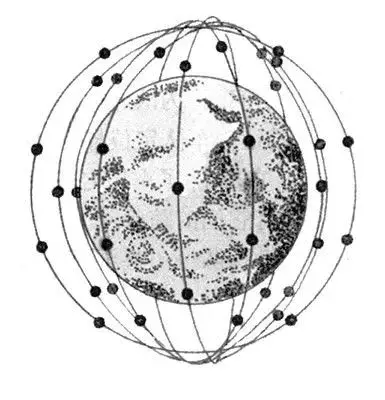
\includegraphics[width=\linewidth]{77.png}
		\caption{铱星计划}
		\label{fig:铱星计划}
	\end{subfigure}
	\caption{摩托罗拉与铱星计划}
	\label{fig:摩托罗拉与铱星计划}
\end{figure}

摩托罗拉的企业文化崇尚技术和创新。当初工程师巴里·伯蒂格因为妻子在加勒比海度假时说她无法用手机联系到她的客户的一句抱怨而产生的突发奇想,得到了当时任公司董事长的加尔文决心把这一计划付诸实践的支持。可见该公司对创新的支持力度之大。然而铱星计划的失败不是技术的失败,只论技术的盲目乐观早已注定了铱星计划要失败。

\section{案例分析}%
\label{sec:案例分析}

\begin{figure}[htpb]
	\centering
	\begin{tikzpicture}[
		start chain=going right,
		node distance=5mm,
		every on chain/.style={
			thick,
			draw=black,
			top color=white,
			bottom color=yellow!40,
			font=\sffamily\small,
			minimum width=6mm,
			minimum height=6mm,
			%drop shadow,
			%label={below:block \tikzchaincount},
		},
		decoration={coil},
		dna/.style={decorate, thick, decoration={aspect=0, segment length=5cm}},
		%    post join/.style={
		%      -stealth,
		%      line width=1.5mm,
		%      red,
		%      rounded corners=1mm,
		%    },
		square/.style={thick,
			draw=black,
			top color=white,
			bottom color=black!10,
			font=\sffamily\small,
			minimum width=12mm,
			minimum height=10mm,
		drop shadow},
		every label/.style={
			font=\sffamily\scriptsize
		},
		]
		\draw[dna, decoration={amplitude=.15cm}] (0,-0) -- (1.1,-0);
		\draw[dna, decoration={amplitude=.35cm}] (1.15,0) -- (1.15,-1.1);
		\draw[dna, decoration={amplitude=.35cm}] (1.15,-1.1) -- (0,-1.1);
		\draw[dna, decoration={amplitude=.35cm}] (0,-1.1) -- (0,0);
		%% Path for dots
		\node [on chain] {优势};
		\node [on chain] {劣势};
		\node [on chain=going below] {机会};
		\node [on chain=going left] {威胁};
	\end{tikzpicture}
	\caption{SWOT模型}
	\label{fig:SWOT模型}
\end{figure}

\begin{description}
	\item[优点]铱星计划从现代电信系统设计的角度来看,是一个符合市场需求的系统。它在总体技术上采用了大量以往的卫星通信系统所未曾采用过的新技术,使得相对传统的基于地球静止轨道的全球移动通信系统而言,铱星移动通信系统在性能、经济、时间和发展等四个方面都达到和保持良好状态,并取得了非常强的竞争优势。从理论上讲,铱星占尽了市场的先机,开创了全球个人通信的新时代,使人们在地球上任何\enquote{能见到天的地方}都可以进行\enquote{无缝隙}的通信联络。它实现了5个\enquote{任何}(即5W):即任何人在任何地点、任何时间与任何人采取任何方式进行通信,被认为是现代通信的一个里程碑。
	\item[缺点]相对地面移动电话系统,铱星系统本身也存在许多不足,手机个头笨重,运行不稳定,价格昂贵,不能在室内和车内使用。而整个世界通信系统的趋势却是手机越做越小,商家为了赚取通话费,甚至无偿赠送手机。
	\item[机会]那些身处偏远地方, 地面无线通信网无法延伸的地方, 如海上石油钻井平台或油轮上工作的人以及那些希望随时随地保持稳定通信的大企业,铱星计划有足够的吸引力。
	\item[威胁]过去十年里地面移动通信发展迅猛,夺走了铱星公司的目标市场,相对地面移动通信,尤其是移动电话领域,铱星计划在时间维上已经失去了市场机会。
\end{description}

\section{总结}%
\label{sec:总结}

根据分析结果,可以得到以下结论:

\begin{description}
	\item[建立完善的组织结构]铱星公司的基本市场运行组织结构是一个由世界上多个辖管地区性 \enquote{闸口} 国家或企业组成的合伙人结构。由于各地区\enquote{闸口}仅负责在本地区范围内的铱星卫星移动通信系统的手持电话的销售和提供相应的服务,各自的利益关系和产权关系极不清晰,导致铱星计划根本无法建立一个面向全球性的市场运营构架。
	\item[正确使用各种内控手段进行调节]之前的分析已经表明摩托罗拉公司的风险评估和预算控制存在严重失策,像风险分析上的盲目乐观,认为用户都属于\enquote{付钱不看账单的一群人}的高层次的国际商务旅行人员。对预算的错误估计导致在系统还未完善的时候就不得不急于推出,而糟糕的用户体验又进一步为之后的失败奠定了祸根。\cite{杨有红2004试论公司治理与内部控制的对接}
	\item[提高财务决策的科学水平]只有提高财务决策的科学水平,才能防止因决策失误而产生的财务风险。正如摩托罗拉公司的发展战略、营销战略制定的严重失误,为之后的财务风险埋下了隐患。企业必须采用科学的决策方法。在决策过程中,应充分考虑影响决策的各种因素,尽量采用定量计算及分析方法,并运用科学的决策模型进行决策,对各种可行方案决策,切忌主观臆断。
	\item[加强管理人员对风险的客观认识]管理者的风险意识也是财务风险相关的一个重要因素。正如摩托罗拉公司的财务危机早有征兆,而管理层却置之不理,最终招来无法挽回的后果。加强风险教育,加强业务培训,提高管理人员素质,提高风险的甄别能力。只有在对财务风险有了一定认识, 在制定决策时考虑到财务风险, 定期对企业各类财务信息加以对比分析, 找出企业潜在的风险因素,才能最大程度避免风险。\cite{孙新宇2016企业财务风险识别与防范案例分析}
\end{description}

% Fakesection 参考文献

\bibliographystyle{IEEEtran}
\bibliography{src/main}

% Fakesection 附录

\appendix

\section{数据}%
\label{sec:数据}

\begin{table}[htpb]
	\centering
	\caption{摩托罗拉资产负债表}
	\label{tab:摩托罗拉资产负债表}
\end{table}
\csvautobooklongtable{src/motorola.csv}

\end{document}

